\documentclass{article}
\usepackage[utf8]{inputenc}
\usepackage{amsmath}
\usepackage{amsfonts}
\usepackage{amssymb}
\usepackage{graphicx}
\usepackage[bookmarks=false]{hyperref}
\usepackage{algorithm}
\usepackage{algpseudocode}
\usepackage{booktabs}

\title{STU-PID: Steering Token Usage via PID Controller for Efficient LLM Reasoning}

\author{
  Aryasomayajula Ram Bharadwaj\\
  \texttt{ram.bharadwaj.arya@gmail.com}\\
  Independent Researcher
}

\begin{document}

\maketitle

\begin{abstract}
Reasoning LLMs trained with long chain-of-thought often overthink, spending
tokens on redundant reflection and transitions that inflate cost without
helping accuracy. Static activation steering (e.g., SEAL) suppresses such
content with a fixed vector but applies the same strength regardless of how
redundant the current chunk actually is. We propose STU-PID, a training-free
decoding-time method that modulates steering strength with a PID controller
driven by a lightweight chunk-level redundancy classifier. On a 100-problem
GSM8K subset with DeepSeek-R1-Distill-Qwen-1.5B, STU-PID improves accuracy
from 81\% to 87\% (+6 pp) while cutting average output length from 1152 to
784 tokens (-32\%).
\end{abstract}

\section{Introduction}

Long chain-of-thought reasoning \cite{wei2022chain} underlies the gains of
o1-style and DeepSeek-R1-style models \cite{guo2025deepseek}, but the same
training signal encourages overthinking: models emit long runs of
reflection and transition text that add cost and sometimes hurt accuracy
\cite{sui2025stop}. Most remedies---length-reward RL, variable-length SFT,
latent-CoT compression---require retraining.

SEAL \cite{chen2025seal} instead steers activations at inference time with a
fixed vector built from the difference between ``execution'' and
``reflection/transition'' chunks. This is cheap and training-free, but the
steering coefficient is a constant: the same push is applied to a chunk that
is clearly redundant and to one that is doing useful work, which can
over-suppress productive reasoning or leave redundancy untouched.

STU-PID closes the loop. A chunk-level classifier estimates the redundancy
probability of the current reasoning chunk, and a PID controller uses the
error between that probability and a target to set the steering coefficient
on the fly. The method is training-free beyond fitting a small linear
classifier and tuning four gains on a validation set.

\textbf{Contributions.}
\begin{itemize}
\item A closed-loop, decoding-time steering scheme that treats activation
      steering as a control problem rather than a fixed intervention.
\item A chunk-level redundancy classifier trained on $\sim$100 labeled
      chunks that serves as the PID feedback signal.
\item On GSM8K (100 problems, DeepSeek-R1-Distill-Qwen-1.5B): +6 pp
      accuracy (81$\to$87\%) and -32\% tokens (1152$\to$784) over the
      unsteered baseline.
\end{itemize}

\section{Related Work}

\textbf{Efficient reasoning.} Sui et al.\ \cite{sui2025stop} survey the
space: length-reward RL, variable-length SFT, latent-CoT compression, and
prompt-level controls. These act at training time or rewrite the reasoning
format; STU-PID acts at decoding time on a frozen model.

\textbf{Activation steering.} SEAL \cite{chen2025seal} categorizes reasoning
chunks as execution, reflection, or transition, and subtracts a fixed
steering vector to suppress the latter two. STU-PID reuses SEAL's vector
construction but replaces the fixed coefficient with a feedback controller,
which is what lets it both improve accuracy and cut tokens rather than
trading one against the other.

\section{Method}

\subsection{Setup}

At decoding step $t$, let $h_t \in \mathbb{R}^d$ be the hidden state at a
chosen layer $l$. Steering replaces $h_t$ with
\[
h'_t = h_t + \alpha_t \cdot v,
\]
where $v$ is a fixed steering direction and $\alpha_t \ge 0$ is a
time-varying coefficient chosen by the controller. Following SEAL
\cite{chen2025seal},
\[
v = \mathbb{E}[h_l \mid \text{redundant chunk}] - \mathbb{E}[h_l \mid \text{required chunk}],
\]
estimated from a small labeled set.

\subsection{Chunk-level redundancy classifier}

We split the generation into fixed-size chunks (24 tokens) and mean-pool
the layer-$l$ hidden states over each chunk. A logistic classifier $C$
trained on $\sim$100 labeled chunks outputs
\[
p_{\text{red},t} = C(\bar h_l^{\text{chunk}(t)}) \in [0,1].
\]
The classifier is the only learned component and its cost is negligible
next to a decoder step.

\subsection{PID controller}

Let $e_t = p_{\text{red},t} - p_{\text{target}}$ be the redundancy error.
The controller maintains
\begin{align*}
I_t &= \mathrm{clip}\bigl(I_{t-1} + K_I e_t,\ -I_{\max},\ I_{\max}\bigr), \\
D_t &= K_D (e_t - e_{t-1}), \\
\alpha_t &= \mathrm{clip}\bigl(\alpha_{t-1} + K_P e_t + I_t + D_t,\ 0,\ \alpha_{\max}\bigr).
\end{align*}
The integral term is clipped to prevent windup, and $\alpha_t$ is floored
at $0$ so the controller can only \emph{push away} from redundancy, never
amplify it. An $\epsilon$-margin on $e_t$ avoids reacting to classifier
noise near the target.

\begin{algorithm}
\caption{STU-PID decoding}
\begin{algorithmic}[1]
\State $\alpha \gets 0$,\ $I \gets 0$,\ $e_{\text{prev}} \gets 0$
\For{generation step $t = 1, 2, \dots$}
  \If{$t \ge t_{\text{init}}$ \textbf{and} within steering window}
    \State $p_{\text{red}} \gets C(\bar h_l^{\text{chunk}(t)})$
    \State $e \gets p_{\text{red}} - p_{\text{target}}$
    \If{$e > \epsilon_{\text{margin}}$}
      \State $I \gets \mathrm{clip}(I + K_I e,\ -I_{\max},\ I_{\max})$
      \State $D \gets K_D (e - e_{\text{prev}})$
      \State $\alpha \gets \mathrm{clip}(\alpha + K_P e + I + D,\ 0,\ \alpha_{\max})$
    \EndIf
    \State $e_{\text{prev}} \gets e$
  \EndIf
  \State $h'_t \gets h_t + \alpha \cdot v$;\quad sample next token from $h'_t$
\EndFor
\end{algorithmic}
\end{algorithm}

\begin{figure}[h]
\centering
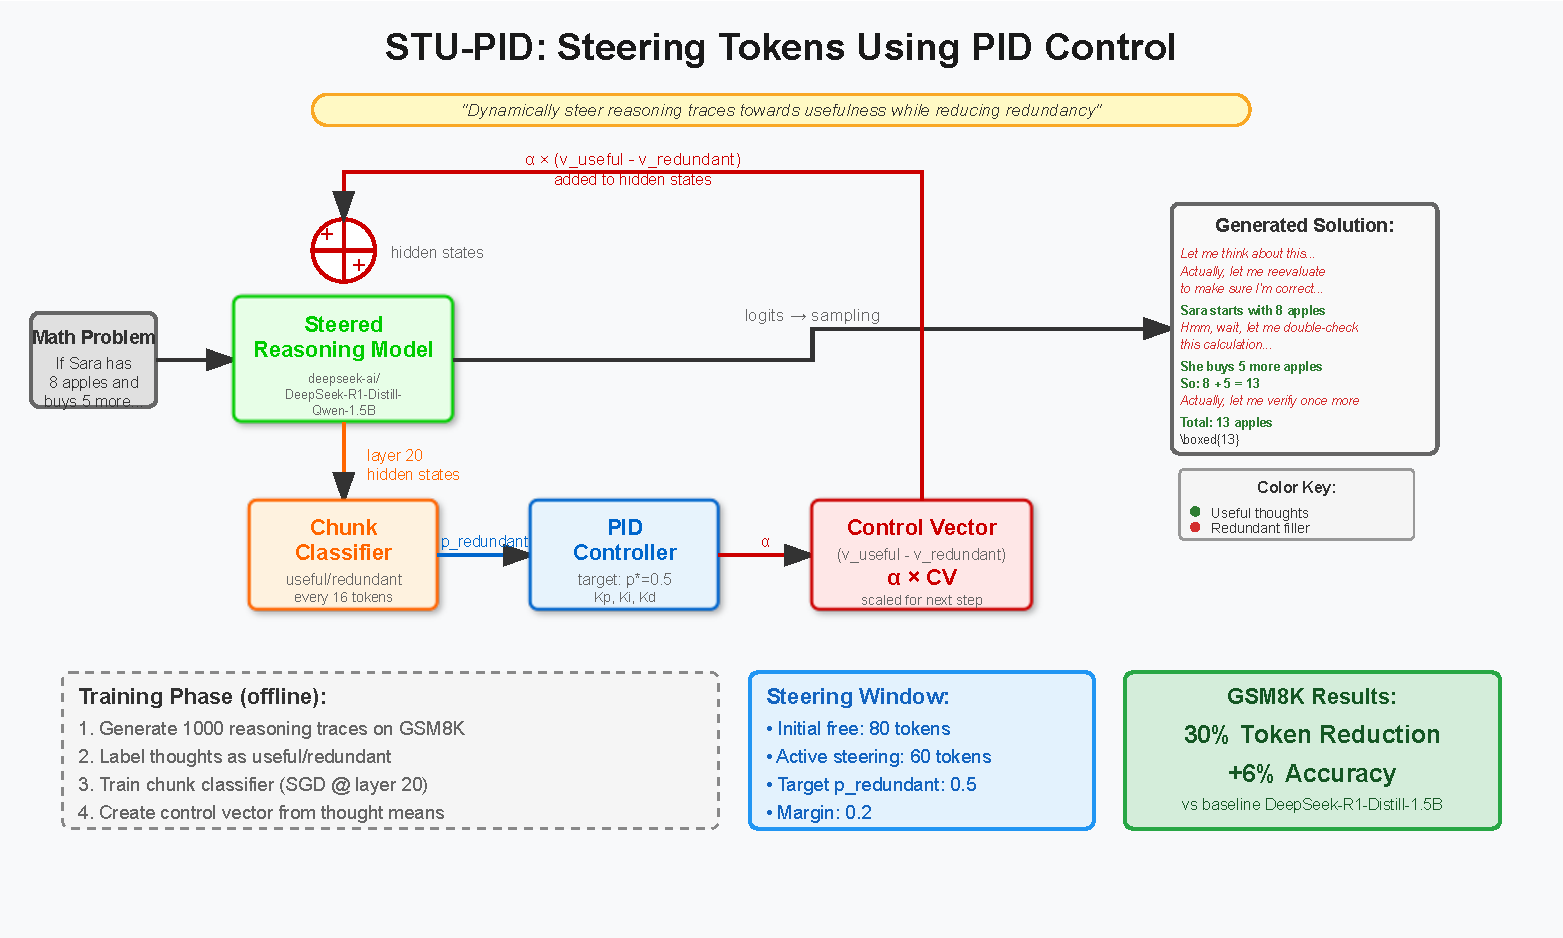
\includegraphics[width=0.95\textwidth]{algo.pdf}
\caption{STU-PID at a glance. The classifier scores each reasoning chunk;
the PID controller turns the redundancy error into a steering coefficient
$\alpha_t$ applied to the layer-$l$ residual stream.}
\label{fig:algorithm}
\end{figure}

\section{Experiments}

\textbf{Model and data.} DeepSeek-R1-Distill-Qwen-1.5B, evaluated on a
100-problem subset of the GSM8K test set.

\textbf{Classifier.} Logistic regression (SGD, log loss) on mean-pooled
layer-20 hidden states; chunk size 24 tokens; trained on $\sim$100 labeled
chunks from GSM8K training problems.

\textbf{Hyperparameters} (tuned on a small held-out set):
$K_P = 0.01$, $K_I = 5\!\times\!10^{-4}$, $K_D = 5\!\times\!10^{-3}$,
$p_{\text{target}} = 0.3$, $\alpha_{\max} = 0.40$, $I_{\max} = 0.20$,
$\epsilon_{\text{margin}} = 0.20$, free period $t_{\text{init}} = 80$
tokens, steering window $60$ tokens, max generation $2048$ tokens.

\textbf{Metrics.} Exact-match accuracy and mean generated tokens per
problem.

\subsection{Main result}

\begin{table}[h]
\centering
\caption{GSM8K, 100 problems, DeepSeek-R1-Distill-Qwen-1.5B.}
\label{tab:main_results}
\begin{tabular}{lcc}
\toprule
Method & Accuracy (\%) & Avg.\ tokens \\
\midrule
Baseline (no steering) & 81.0 & 1152 \\
STU-PID                & 87.0 &  784 \\
\bottomrule
\end{tabular}
\end{table}

STU-PID improves accuracy by 6 percentage points while using 32\% fewer
tokens (Table~\ref{tab:main_results}). Both metrics move in the same
direction, which is the main empirical point: adaptive steering can
suppress redundancy without the accuracy cost that a constant coefficient
incurs when it is strong enough to be useful on the worst chunks.

\section{Limitations}

The evaluation covers 100 problems, one dataset, and one 1.5B model, so
the numbers should be read as a proof of concept rather than a benchmark
result. The classifier is trained on math chunks and is unlikely to
transfer to non-math reasoning without new labels. PID gains and the
target $p_{\text{target}}$ were tuned by hand on a small set; behavior
under automated tuning or larger models is not yet characterized. We also
do not ablate the PID terms individually, so the relative contribution of
$K_P$, $K_I$, and $K_D$ is unknown.

\section{Conclusion}

STU-PID turns activation steering into a closed-loop control problem: a
small redundancy classifier supplies feedback, and a PID controller sets
the steering coefficient per chunk. On a 100-problem GSM8K slice with
DeepSeek-R1-Distill-Qwen-1.5B, this replaces a $+$accuracy$/-$tokens
tradeoff with a $+$accuracy$/+$token-savings improvement (81$\to$87\%,
1152$\to$784 tokens). Whether the approach holds up at larger scale and on
non-math reasoning is the obvious next question.

\noindent Code and results: \url{https://github.com/arambharadwaj/pid_steering}

\begin{thebibliography}{10}

\bibitem{wei2022chain}
Jason Wei, Xuezhi Wang, Dale Schuurmans, Maarten Bosma, Brian Ichter, Fei Xia, Ed Chi, Quoc Le, and Denny Zhou.
Chain-of-thought prompting elicits reasoning in large language models.
\textit{arXiv preprint arXiv:2201.11903}, 2022.

\bibitem{guo2025deepseek}
Daya Guo, Dejian Yang, Haowei Zhang, Junxiao Song, Peiyi Wang, et al.
DeepSeek-R1: Incentivizing reasoning capability in LLMs via reinforcement learning.
\textit{arXiv preprint arXiv:2501.12948}, 2025.

\bibitem{sui2025stop}
Yang Sui, Yu-Neng Chuang, Guanchu Wang, Jiamu Zhang, Tianyi Zhang, Jiayi Yuan, Hongyi Liu, Andrew Wen, Shaochen Zhong, Na Zou, Hanjie Chen, and Xia Hu.
Stop overthinking: A survey on efficient reasoning for large language models.
\textit{arXiv preprint arXiv:2503.16419}, 2025.

\bibitem{chen2025seal}
Runjin Chen, Zhenyu Zhang, Junyuan Hong, Souvik Kundu, and Zhangyang Wang.
SEAL: Steerable reasoning calibration of large language models for free.
\textit{arXiv preprint arXiv:2504.07986}, 2025.

\end{thebibliography}

\end{document}
